\begin{ejercicio}
	Solución: Para el estado
		$$ \ket{S_n +} = \frac{\sqrt{3}}{2} \ket{+} + \frac{i}{2} \ket{-}. $$
	\begin{enumerate}[a)]
		\item El estado ya se encuentra respecto a la base $\alpha$.
		\item El bra sería
			$$ \bra{S_n +} = \frac{\sqrt{3}}{2} \bra{+} - \frac{i}{2} \bra{-}. $$
		\item Tomando $\ket{S_x +} = \frac{1}{\sqrt{2}} \ket{+} + \frac{1}{\sqrt{2}} \ket{-} $, encontramos la probabilidad de medir $+\frac{\hbar}{2}$
			$$ \abs{\braket{S_x +}{S_n +}}^2 = \frac{1}{2} = 50\% . $$
		\item Realizamos lo mismo que en el inciso anterior con $\ket{S_y -} = \frac{1}{\sqrt{2}} \ket{+} - \frac{i}{\sqrt{2}} \ket{-}$. Entonces
			$$ \abs{\braket{S_y -}{S_n +}}^2 = 0.0669873 = 6.699\% . $$
		\item Utilizando la matriz de cambio de base vista en clase
			$$ Q = \frac{1}{\sqrt{2}} \mqty(1 & -i \\ 1 & i), $$
			Encontramos el estado $\ket{S_n +}$ en términos de la base $\gamma$. Encontramos el vector $(\ket{S_n +})_\gamma$ en términos de la base resolviendo el siguiente sistema
			$$ \frac{a}{\sqrt{2}} \mqty(1 \\ i) + \frac{b}{\sqrt{2}} \mqty(1 \\ -i) = \mqty(\flatfrac{\sqrt{3}}{2} \\ \flatfrac{i}{2}). $$
			Con lo que encontramos al estado
			$$ \qty(\ket{S_n +})_\gamma = \frac{\sqrt{6} + \sqrt{2}}{4} \ket{S_y +} + \frac{\sqrt{6} - \sqrt{2}}{4} \ket{S_y -}. $$
		\item Teniendo $\ket{\psi _o} = \ket{S_n +}$ y el operador evolución $U(t) = e^{-\frac{it}{\hbar} H} = e^{-\frac{it}{\hbar} \omega S_z}$. Aplicando $\ket{\psi (t)} = U(t) \ket{\psi _o}$, entonces
			$$ \ket{\psi (t)} = \frac{\sqrt{3}}{2} e^{-\frac{it}{\hbar} \omega S_z} \ket{+} + \frac{i}{2} e^{-\frac{it}{\hbar} \omega S_z} \ket{-} = \frac{\sqrt{3}}{2} e^{-\frac{i\omega t}{2}} \ket{+} + \frac{i}{2} e^{\frac{i\omega t}{2}} \ket{-}. $$
		\item Con el resultado anterior, valuamos en un tiempo $t = \flatfrac{\pi}{\omega}$.
			$$ \ket{\psi \qty(\frac{\pi}{\omega})} = -\frac{i\sqrt{3}}{2} \ket{+} - \frac{1}{2} \ket{-}. $$ 
	\end{enumerate}
\end{ejercicio}




\begin{ejercicio}
	Solución: 
	\begin{enumerate}[a)]
		\item Aplicando el operador evolución al estado $\ket{\psi _o} = \ket{S_y +}$, se tiene
			$$ \ket{\psi (t)} = U(t) \ket{\psi _o} = \frac{1}{\sqrt{2}} e^{-\frac{i\omega t}{2}} \ket{+} + \frac{i}{\sqrt{2}} e^{\frac{i\omega t}{2}} \ket{-} = \frac{1}{\sqrt{2}} \ket{+} + \frac{i}{\sqrt{2}} e^{i\omega t} \ket{-}. $$
		\item El bra sería
			$$ \bra{\psi (t)} = \frac{1}{\sqrt{2}} \bra{+} - \frac{i}{\sqrt{2}} e^{-i\omega t} \bra{-} $$
		\item Para un $t = \frac{\pi}{\omega}$, se tiene
			$$ \ket{\psi \qty(\frac{\pi}{\omega})} = \frac{1}{\sqrt{2}} \ket{+} - \frac{i}{\sqrt{2}} \ket{-} = \ket{S_y -} . $$
		\item Para $t = \frac{2\pi}{\omega}$
			$$ \ket{\psi \qty(\frac{2\pi}{\omega})} = \frac{1}{\sqrt{2}} \ket{+} + \frac{i}{\sqrt{2}} \ket{-} = \ket{S_y +} . $$
		\item Ya se demostró en los dos incisos anteriores.
		\item Gráficamente,
			\begin{figure}[H]
				\centering
				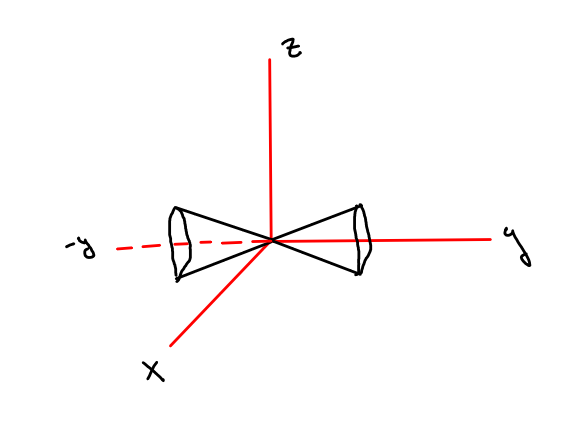
\includegraphics[scale=0.5]{./img/p2f.png}
				\caption{Podemos visualizar, en el eje $y$ positivo, los estados $\ket{\psi _o}$ y $\ket{\psi (\flatfrac{2\pi}{\omega})}$; mientras que en el eje $y$ negativo, visualizamos $\ket{\psi (\flatfrac{\pi}{\omega})}$.}
				\label{p2f}
			\end{figure}
		\item Utilizamos el módulo de funciones para encontrar $\expval{S_y}{\psi (t)}$, lo que nos da
			$$ \expval{S_y} = \frac{\hbar}{4} \qty(e^{i\omega t} + e^{i\omega t}) = \frac{\hbar}{2} \cos{\omega t}. $$
	\end{enumerate}
\end{ejercicio}




\begin{ejercicio}
	Sabiendo que para las matrices de pauli se cumple que
		$$ [\pauli{j} ,\pauli{k}] = 2i\varepsilon _{jkl} \pauli{l}, $$
	donde $\varepsilon_{jkl}$ es el tensor de Levi$-$Civita. Entonces, sabiendo que los operadores en cada eje están definidos como $S_x = \frac{\hbar}{2} \pauli{x}$, $S_y = \frac{\hbar}{2} \pauli{y}$ y $S_z = \frac{\hbar}{2} \pauli{z}$, entonces, reemplazando valores y utilizando la función \texttt{LeviCivitaTensor[3]} para encontrar los respectivos valores del mismo.
		$$ [S_x,S_z] = 2\qty(\frac{\hbar ^2}{4}) i \varepsilon_{xzy} \pauli{y} = \mqty(0 & -\frac{\hbar ^2}{2} \\ \frac{\hbar ^2}{2} & 0), $$
		$$ [S_y,S_z] = 2\qty(\frac{\hbar ^2}{4}) i \varepsilon_{yzx} \pauli{x} = \mqty(0 & \frac{i\hbar ^2}{2} \\ \frac{i\hbar ^2}{2} & 0). $$
\end{ejercicio}




\begin{ejercicio}
	Solución: Teniendo que los operadores escalera se definen como
		$$ S_+ = \hbar \mqty(0 & 1 \\ 0 & 0), \qquad S_- = \hbar \mqty(0 & 0 \\ 1 & 0). $$
		Y que $\ket{S_y +} = \frac{1}{\sqrt{2}} \mqty(1 \\ i)$ y $\ket{S_y -} = \frac{1}{\sqrt{2}} \mqty(1 \\ -i)$
	\begin{enumerate}[a)]
		\item $$ S_+ \ket{S_y +} = \hbar \mqty(\frac{i}{\sqrt{2}} \\ 0). $$
		\item $$ S_+ \ket{S_y -} = \hbar \mqty(-\frac{i}{\sqrt{2}} \\ 0). $$
		\item $$ S_- \ket{S_y +} = \hbar \mqty(0 \\ \frac{1}{\sqrt{2}}). $$
		\item $$ S_- \ket{S_y -} = \hbar \mqty(0 \\ \frac{1}{\sqrt{2}}). $$
	\end{enumerate}
\end{ejercicio}















%%%%%